\setlength{\parskip}{1em}
\setlength{\parindent}{0em}

\section{How to Evaluate Models}

Currently, we try to find the best parameters by visually inspecting the fit:
\begin{enumerate}
\item We start by plotting the \emph{predicted} and \emph{actual} values according to the model
\item We can break this down further using a different \emph{color} for each gender
\item We can color by age, and \emph{wrap} by gender to make this clearer
\end{enumerate}
Note: \emph{Discrete variables} (such as gender) are automatically colored with a discrete color scale, while \emph{continuous variables} (such as age) are automatically colored with a continuous color scale.

\section{Modeling Variability}

However, all this is done by summarizing the \emph{average} of each gender/age combination, which might cause us to overlook some variability in our observations. For instance, plotting every point shows that variability \emph{within} age is higher than variability \emph{across} age in the figure below), which reveals the deficiencies of our model.

\begin{figure}[h]
\begin{center}
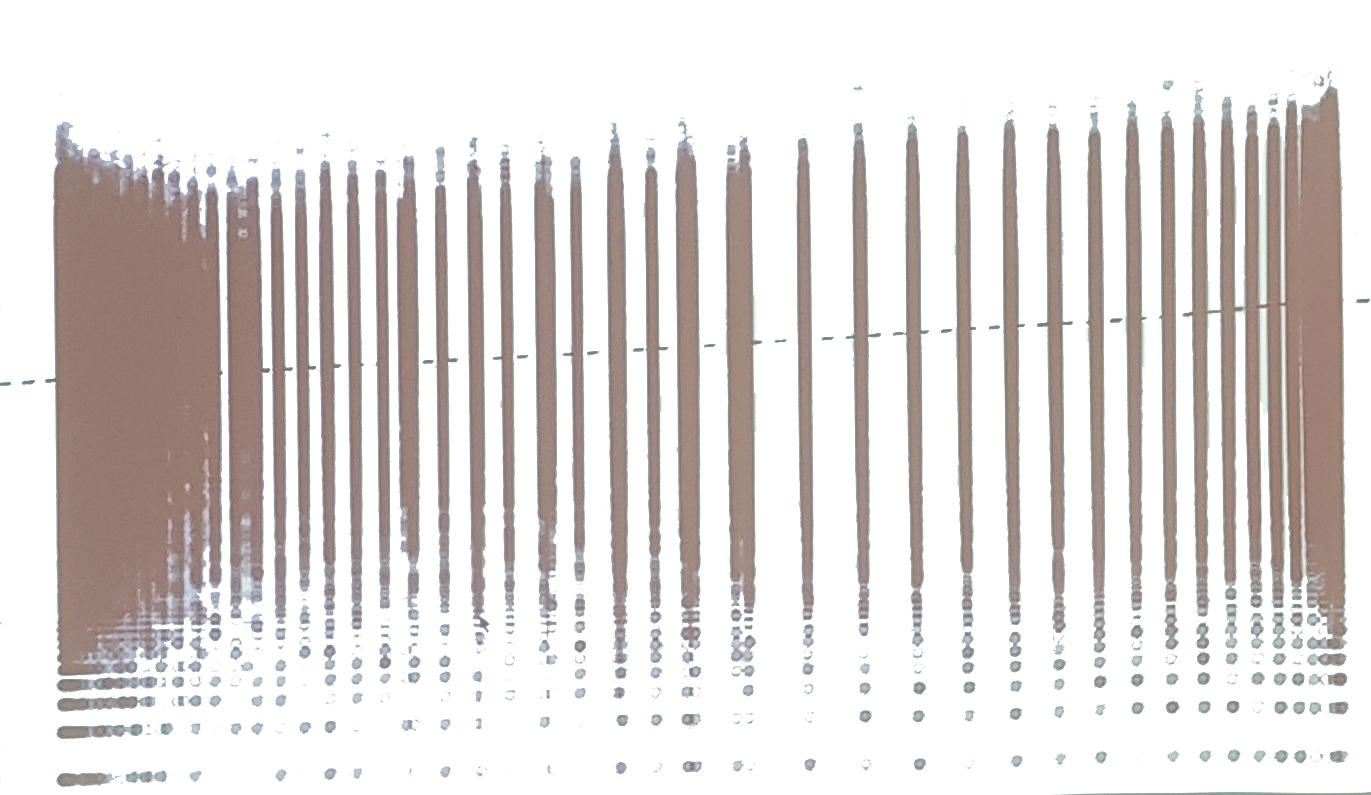
\includegraphics[width=0.5\textwidth]{ClassFigure.jpg}
\caption{Complete Plot of Observations}
\end{center}
\end{figure}
\small{Source: Class notes, Jake Hofman}

Traditional methods of reporting statistics (by significance value) also overlook this variability, because while it is true that you have explained average changes by age, it is also true that you have \emph{not} explained the rest of the variability in the model. In other words, we can explain \emph{collective} trends, but not \emph{individual} observations that we might see in the real world.

There might also be \emph{unexplored transformations} to the data that might reduce this variability, or \emph{other variables} such as internet connection that have not been recorded.

\section{How Good is a Model?}

There are two main metrics we can use to evaluate the fit of a model:
\begin{itemize}
\item Root mean squared error (RMSE)\[\sqrt{\frac{1}{N}\sum_{i}^{N}(y_i-\hat{y})^2}\]\begin{itemize}
\item R syntax: \texttt{sqrt(mean((pred\ -\ actual)\^{}2)))}
\item We take the square root because we are calculating the squared difference between predicted and observed values.
\item To obtain a baseline MSE, we calculate the difference between the each observation and the mean of the observed data (i.e.~the variance of y).
\item We then compare this to the MSE of the model with \[\frac{MSE_{baseline} - MSE_{model}}  {MSE_{baseline}} = R^2\] where \(R^2\) is also the fraction of variance explained.
\end{itemize}
\item Pearson's correlation coefficient \[\frac{\sum_i(y_i-\bar{y})(\hat{y_i}-\hat{\bar{y}})}{[\sum_i(y_i-\bar{y})^2]^\frac{1}{2}[\sum_i(\hat{y_i}-\hat{\bar{y}})^2]^\frac{1}{2}}\]\begin{itemize}
\item R syntax: \texttt{cor(pred,\ actual)}
\item We calculate the deviations from the mean of observed and actual data, and then scale them accordingly by the denominator
\item The square of Pearson's correlation coefficient is also equal to to \(R^2\) in the MSE, or the fraction of variance explained.\end{itemize}
\end{itemize}

Applying the above tools to our previous model, we get a low \(R^2\) of 0.019, which shows that our model in fact explains \emph{very little} of the data. However, we need to remember that MSE is also highly susceptible to outliers, because a big difference between predicted and actual outcomes may skew the results.

\section{Explaining the Past vs. Predicting the Future}

As we add degrees to a polynomial, we add accuracy to the predictive power of a model because of the increased flexibility. The \texttt{poly(x,\ degree,\ raw=true)} function in R automatically adds successive polynomial transformation (until a user-defined k degree) of a variable to a linear model. We need to remember to remove the original variable, because this transformation will also give results for \texttt{k=1}.

However, while this succeeds in predicting the \emph{past}, it does not necessarily have a bearing on how accurately we predict the \emph{future}. Polynomial transformations also increase variability in our results, such that different observation sets might lead us to drastically different conclusions (see \emph{Bias and Variance}).

Our models should thus be \emph{complex} enough to explain the past, but \emph{simple} enough to generalize the future. We can achieve this by randomly splitting our data into three sets: training set, validation 
set, and testing set. \begin{enumerate}
\item Fit the models based on the \emph{training set}
\item Use the \emph{validation set} to evaluate their performance
\item Quote final performance on the \emph{testing set} \end{enumerate}

If the model does not perform well on the testing set, we should not amend it using the same dataset, but wait for new data to come in. Unfortunately, this is often ignored in practice. A possible solution is a \emph{reusable holdout set} which adds noise to the results of the testing set, rather than revealing the testing data directly.

\section{Bias and Variance}

As discussed earlier, polynomial models have \emph{high variance} because different observation sets can lead to drastically different predictions. However, there is often a tradeoff between variance (predictiveness of model with \emph{different} observations) and bias (predictiveness of model with \emph{more} observations).

Loosely speaking, the relationship between variance and bias can be captured in the following equation, such that for a given MSE (and irreducible error), an increase in bias will result in a decrease in variance (or vice versa).

\[MSE = Bias^2 + Variance + Irreducible Error\]

While a linear model is \emph{low variance}, it is likely to be \emph{high bias} because there are no guarantees that the relationship is indeed linear. In other words, even with infinite observations, a model may still be wrong. By contrast, a n-degree polynomial model is likely to be \emph{low bias}, because with infinite observations we are more likely to arrive (trivially) at an accurate representation of the world.

A \emph{generalization curve} evaluates the complexity of the model based on its predictive power on the training sample and test sample. Using this, we can identify a point of divergence between the two lines to find a middle ground between bias and variance.

\begin{figure}[h]
\begin{center}
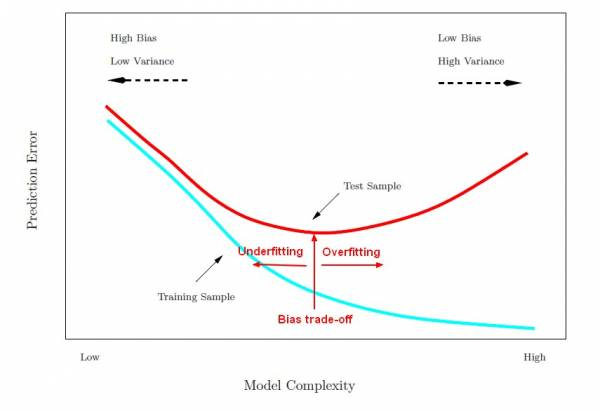
\includegraphics[width=0.5\textwidth]{GeneralizationCurve.jpg}
\caption{Generalization Curve for Training and Testing/Validation Errors}
\end{center}
\end{figure}

\small{Source: \url {http://gerardnico.com/wiki/_media/data_mining/model_complexity_error_training_test.jpg}}

\section{Choosing the Training and Validation Sets}

When shuffling the data, we can use the \texttt{sample()} function in R to select the indices of observations we want to include in either the training or test sets. However, we need to be careful of inherent orderings in the data, which might contain trends (e.g. seasonality) that would be incorrectly eliminated by random sampling.

We notice, however, that our results can vary significantly based on our assignment of the training and validation sets, which brings us to \emph{K-fold cross validation}, which involves taking different subsets of training and validation data such that every observation is at one point part of the validation set. We can then average across all the runs to find the best possible model.

To process this in R, we simply create a variable called \texttt{num\_folds} and call \texttt{sample(1:num\_folds)} to split the folds evenly between the observations. We also keep track of both the average test error and standard error across all the folds, to help us evaluate the significance of any reduction in observed error.

\begin{figure}[h]
\begin{center}
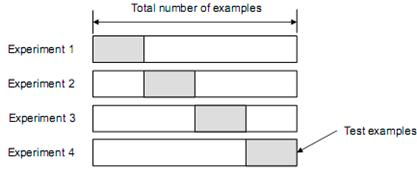
\includegraphics[width=0.5\textwidth]{KFolds.jpg}
\caption{4-Folds Cross Validation with Training and Testing/Validation Sets}
\end{center}
\end{figure}

\small{Source: \url{http://www.imtech.res.in/raghava/gpsr/Evaluation_Bioinformatics_Methods_files/image002.jpg}}

\section{Regularization}

\emph{Regularization} involves penalizing complexity in our loss
function for a specific choice to map it in the model. We can do so using either Ridge Regularization or Lasso Regularization. \begin{itemize}
\item Ridge Regularization \[\mathcal{L}=\frac{1}{n}\sum_i^n(y_i-wx_i)^2+\lambda \vert\vert w\vert\vert^2\]As \(\lambda\) increases, the coefficients decrease which reduces the weighting of the model fit.
\item Lasso Regularization \[\mathcal{L}=\frac{1}{n}\sum_i^n(y_i-wx_i)^2+\vert\vert w_1\vert\vert+\vert\vert w_2\vert\vert+...\] This effectively performs variable selection by ignoring near-zero coefficients.
\end{itemize}

